\section{Motivation}

To introduce control systems, let's consider a very simple physical system:
a train moving along a 1-dimensional railway. If the train moves with
constant acceleration $a$, and at $t=0$ it's position and velocity
are $x_0$ and $v_0$ (respectively), it's motion is given by the solution
to the following ODE:

\begin{equation}
    \label{eq:train_cte}
    \begin{cases}
        x''(t) = a\\
        x(0) = x_0\\
        x'(0) = v_0
    \end{cases}
\end{equation}
\\

However, in reality, trains very rarely move with constant acceleration: usually,
theres a conductor controlling how the train moves. To consider a very simplified
model, let's say that, at any instant $t$, the conductor can choose
the acceleration $a(t)$ of the train, with the constraint $|a|\leq 1$.
We denote by $u: \real \to [-1,1]$
the function $t \mapsto a(t)$, which will be called the \textit{control function}.
The equation
of motion of the train now becomes:

\begin{equation}
    \label{eq:train_ctrl}
    \begin{cases}
        x''(t) = u(t)\\
        x(0) = x_0\\
        x'(0) = v_0
    \end{cases}
\end{equation}
\\

If $u: \real \to [-1,1]$ is well-behaved enough (see \autoref{apdx:EDOs}),
we can find a unique $x : I \subseteq \real \to \real$ that solves
this equation almost everywhere. This class of well-behaved
functions will be the \textit{admissible control functions}.
An important subset of the admissible control functions is the
class of \textit{piecewise constant function}, that is, functions
$u: \real \to [-1,1]$ such that there is a collection of intervals
covering $\real$ with $u$ being constant in the interior of each such interval.

\begin{figure}[H]
    \centering
    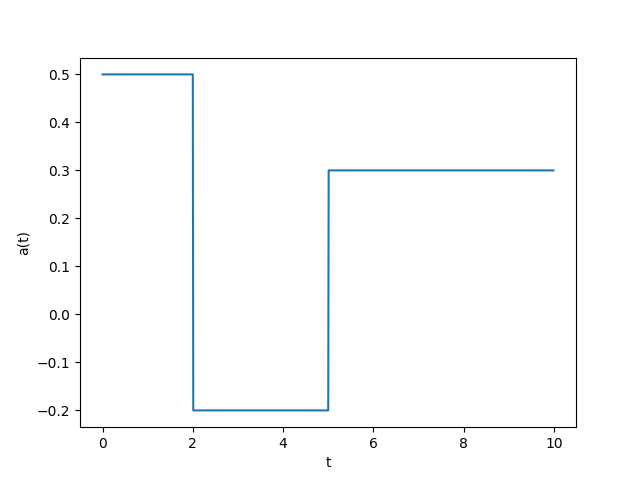
\includegraphics[scale = 0.5]{graf/piecewisecte.png}
    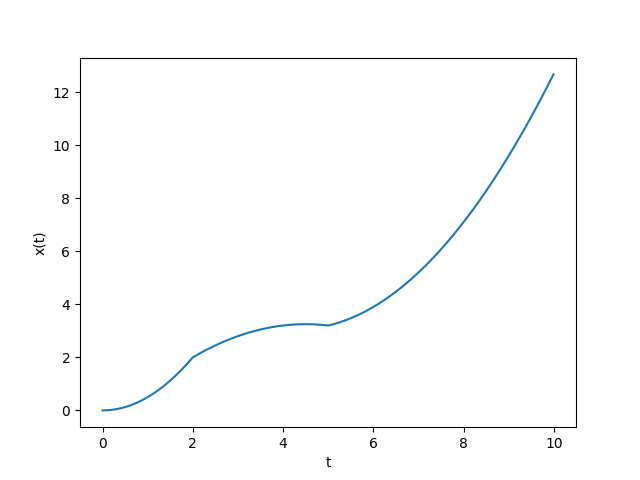
\includegraphics[scale=0.5]{graf/piecewisecte_sol.png}
    \caption{An exemple of a piecewise constant $u(t)$,
    and the corresponding solution $x(t)$ for
    $x_0=v_0=0$}
    \label{fig:piecewise_cte}
\end{figure}

The equation $x'' = u$ (with the constraint $|u| \leq 1$) is
an exemple of a \textit{control system} with \textit{control parameter}
$u$.
We will define precisely what this is later. For now, let's focus on what we
can do with a control system.

The possibility
of choosing the function $u$, and therefore the evolution
of the system represented by \autoref{eq:train_ctrl},
gives rise to many interesting problems, for exemple:

\begin{itemize}
    \item Given an initial state $(x_0, v_0)$, can we choose an admissible
    $u$ such that we eventually reach
    another state $(x_1, v_1)$? (If this is the case, we say that
    $(x_1, y_1)$ is reachable from $(x_0,v_0)$)

    \item Given an initial state $(x_0, v_0)$ and another state
    $(x_1, v_1)$ reachable from $(x_0,v_0)$,
    is there an admissible $u$ that minimizes
    the time we take to go from $(x_0,v_0)$ from $(x_1,v_1)$?
    If this is the case, how can we find such $u$?

    \item Given an initial state $(x_0, v_0)$ and another state
    $(x_1, v_1)$ reachable from $(x_0,v_0)$,
    is there an admissible $u$ that minimizes
    the amount of work we make to go from $(x_0,v_0)$ from $(x_1,v_1)$?
    If this is the case, how can we find such $u$?

\end{itemize}

In this simple exemple (and considering only piecewise constant controls),
all of those question can be answered using rather elementar
techiniques.

Let's now express our system in the language
of differential geometry to shed some
light on how we will approach control systems. 

We use
the usual trick to reduce the order of \autoref{eq:train_cte}
from $2$ to $1$. Consider the plane $\real^2$ with coordinates
$(y^1,y^2)$. Given $x : I \subseteq \real \to \real$ and $a \in \real$,
we define $q: I \to \real^2$ and $X_a:\real^2 \to \real^2$
by $q(t) = (x(t), x'(t))$, $X_a(y^1,y^2) = (y^2, a)$.
\autoref{eq:train_cte} can now be expressed as:

\begin{equation}
    \label{eq:train_field}
    \begin{cases}
        q'(t) = X_a(q(t))\\
        q(0) = (x_0, v_0) = q_0
    \end{cases}
\end{equation}

Notice that the solution to the equation above is completly determined by the vector
field $X_a \in \X(\real^2)$ and the initial condition
$q_0 \in \real^2$.

The control system expressed by the equation $x'' = u$
can now be expressed as $q' = X_u(q)$. The space
of possible values for the control parameter $u$, namely $U = [-1,1]$, is called
the \textit{space of control parameters}. Our
control system now can be sythesised as the (parametrized) family
of vector fields $\{X_u\}_{u \in U}$, each determining an ODE with which
our system can evolve.



\section{So... What is a control system?}
